\documentclass[a4paper, 10pt]{article}
\usepackage{graphicx}
\usepackage[margin = 1in]{geometry}
\usepackage{parskip}
\usepackage[hidelinks, colorlinks = true, citecolor = black, linkcolor = blue]{hyperref}
\usepackage{amsmath}
\usepackage{tabularx}
\usepackage{csvsimple}
\usepackage{subcaption}
\newcommand{\inv}{^{\raisebox{.2ex}{$\scriptscriptstyle-1$}}}

\begin{document}
\begin{flushleft}
\section{Introduction}
The aim of this lab is to measure the spring constant of a helical spring and to
compare it to the theoretical value. Afterwards, the period of vibration will also be
measured, while also measuring the effect of spring mass on this value.
\section{Theory}
Hooke's law, as defined by the 17th century physicist Robert Hooke, states that
the force exerted by a spring is directly proportional to the elongation or
compression of the spring.
\par
A helical spring is a part of wire coiled or wound in the shape of a helix. When
a spring with the spring constant $k$ and the unstretched length $l_0$ is
stretched or compressed to the length $l_e$, the force exerted by the spring
will be a relation between $k$ and $\Delta l$. For small deflections Hooke's law
is formulated in Equation 1.
%refr
\par
\begin{equation}
    F_e = -kx = -k(l_e - l_0)
\end{equation}
Where:
\begin{itemize}
    \item $F_e$ is the force exerted by the spring
    \item $k$ is the spring constant
    \item $x$ is the displacement
    \item $l_e$ is the stretched length of the spring
    \item $l_0$ is the unstretched length of the spring
\end{itemize}
Considering an ideal spring, we mount a system made of a helical spring and a
mass at the end vertically, where it gets to an equilibrium position. The force
of the spring in the equilibrium position is equal to the weight force of the
object.
\par
\begin{equation}  \label{eq:2}
    k x_e = mg 
\end{equation}
When displacing the mass from the equilibrium position, the system will start
oscillating.
Using Newton's second law, Equation 3 is determined.
\begin{align} 
    m \frac{d^2 x}{d t^2} &= mg - kx = mg - k (x_e + x^{\prime}) \\
\intertext{Since:} \nonumber \\   
    k x_e &= Cst \nonumber \\ 
    \frac{d^{\,2} x}{d t^2} &= \frac{d^2 x^{\prime}}{d t^2} \text{($x_e$ is constant, $x = x_e + x^\prime$)} \nonumber
\intertext{The equation becomes:} \nonumber \\
    \frac{d^{\,2} x^{\prime}}{d t^2} &= -\frac{k}{m}x^{\prime} \label{eq:4}
\end{align}
Where $x^{\prime}$ is the position relative to the equilibrium position.
\newpage
Solving the differential equation, Equation~\ref{eq:4} an expression for the relative
position is found:
\begin{equation}
    x^{\prime}(t) = Acos(\sqrt{\frac{k}{m}}t + \Phi)
\end{equation}
Where:
\begin{itemize}
    \item $x^{\prime}(t)$ is the position relative to the equilibrium position
    \item $A$ is the amplitude
    \item $\Phi$ is the phase angle~(constant value that depends on initial conditions)
\end{itemize}
\par
The time period is given by Equation~\ref{eq:6}:
\begin{equation} \label{eq:6}
    T_{id} = 2 \pi \sqrt{\frac{m}{k}}
\end{equation}
However, since the impact of the spring's weight cannot be ignored, the formulas
have to be modified to include the moment of inertia, which affects k. To
account for this, the corrected formula is used:
\begin{equation}
    T_{cor} = 2 \pi \sqrt{\frac{m+\frac{m_S}{3}}{k}}
\end{equation}
These formulas are used to validate Hooke's law and determine the spring
constant. The corrected formula for period can also be used to compare
measurements to theoretical values.
\section{Method and Materials}
\subsection{Experimental setup}
The setup for the experiment consists of a spring mounted to a vertical stand
and a ruler next to the spring. Weight is added progressively, changing
displacements to accurately calculate the spring constant. The mass is measured
using a digital scale, displacement is measured with a ruler and the period is
measured using a chronometer. Figure 1 shows the experimental setup.
\begin{figure}[!h]
    \centering
    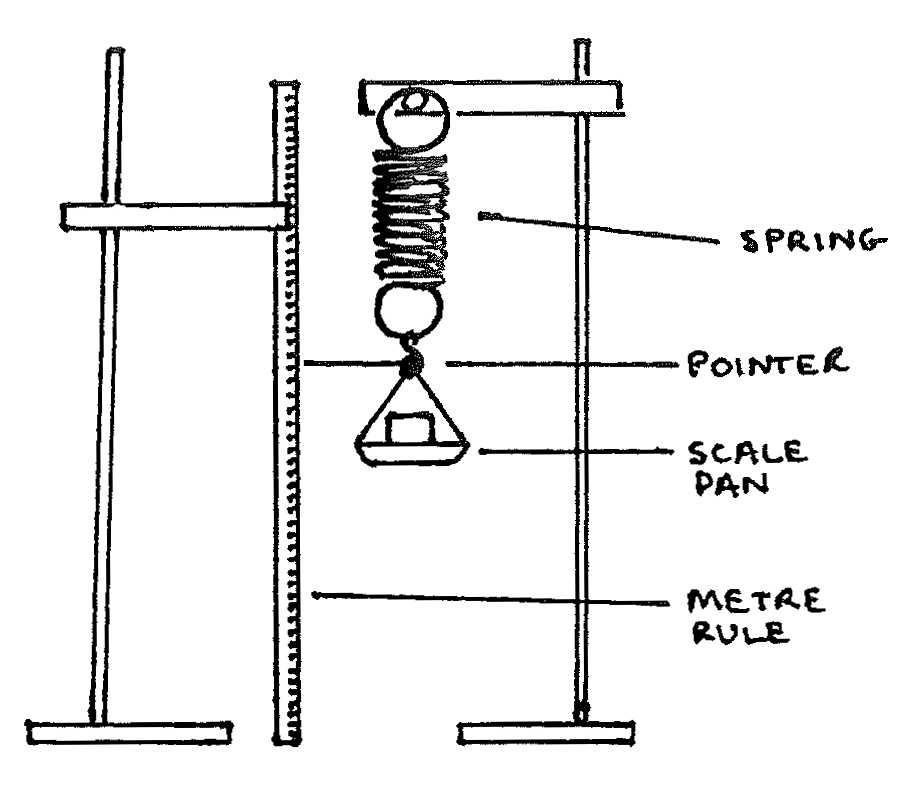
\includegraphics[width = 0.5\linewidth]{13.png}
    \caption{Drawing of the experiment setup(reft)}
\end{figure}
\newpage
\subsection{Measuring instruments}
\begin{itemize}
    \item Vertical meter ruler with 1mm increment ($\pm 0.5~\mathrm{mm}$ uncertainty)
    \item Digital scale ($\pm 0.01~\mathrm{g}$ uncertainty)
    \item Helical spring
    \item Smartphone used as chronometer ($\pm  0.01~\mathrm{s} $)
    \item Spring stand
\end{itemize}
\subsection{Method}
For the first experiment, the spring is attached to the vertical stand with a ruler by its side. Weights
with known mass are added to the spring, measuring the elongation which are used
to calculate the spring constant $k$.
\par
For the second experiment, weights are attached to the spring, the weights
are displaced and the time for 30 oscillations to happen is measured three
times. By repeating the experiment with multiple masses, the theoretical values
can be more accurately compared to the experimental results.
\section{Results spring constant}
\subsection{Measurements}
The measured values for the mass of the holder plus discs $m$, the unstretched
length $l_0$, the stretched length $l_1$, the elongation $x_e$ and the spring
constant $k$ for both the short and long spring are described in tables 1 and 2.
\begin{table}[!h]
    \centering
    \caption{Measurements for the short spring}
    \label{tab:1}
    \begin{tabular}{|c|c|c|c|c|c|c|} 
    \hline
    mass of discs [g] & $l_0$ [cm] & $l_1$ [cm] & $x_e$ [m] &
    $mg$ [N]  & $k$ [$\mathrm{Nm\inv}$] & $\Delta k$ [$\mathrm{Nm\inv}$]  \\ 
    \hline
    31.1                              & 4.7     & 13.1    & 0.08   & 0.31 & 3.63     & 0.16    \\ 
    \hline
    52.1                              & 4.7     & 18.5    & 0.14   & 0.51 & 3.70     & 0.10    \\ 
    \hline
    70.8                               & 4.7     & 24.4    & 0.20   & 0.69 & 3.53     & 0.07    \\ 
    \hline
    91.9                               & 4.7     & 29.95   & 0.25  & 0.90 & 3.57     & 0.05   \\ 
    \hline
    110.46                             & 4.7     & 35.4    & 0.31   & 1.08 & 3.53     & 0.05     \\
    \hline
    \end{tabular}
\end{table}
\begin{table}[!h]
    \centering
    \caption{Measurements for the long spring}
    \begin{tabular}{|c|c|c|c|c|c|c|} 
    \hline
    mass of the discs [g] & $l_0$ [cm] & $l_1$ [cm] & $x_e$ [m] & $mg$ [N]  &
    $k$ [$\mathrm{Nm\inv}$] & $\Delta k$ [$\mathrm{Nm     \inv}$]        \\ 
    \hline
    31.14                 & 17.35   & 18.7    & 0.014 & 0.31 & 22.63      & 5.93  \\ 
    \hline
    52.14                 & 17.35   & 19.7    & 0.024 & 0.51 & 21.77     & 3.27 \\ 
    \hline
    70.8                  & 17.35   & 20.65   & 0.033  & 0.69 & 21.05     & 2.26  \\ 
    \hline
    91.9                  & 17.35   & 21.6    & 0.043 & 0.90 & 21.21     & 1.77  \\ 
    \hline
    110.46                & 17.35   & 22.7    & 0.054 & 1.08 & 20.25     & 1.34  \\
    \hline
    \end{tabular}
\end{table}
\newpage
\subsection{Graphs}
By plotting the values in Tables 1 and 2, the spring constant of each spring can
be determined. A graph for each spring, with the weight as a function of elongation is plotted,
is shown in Figures 2 and 3.
\begin{figure}[!h]
    \centering
    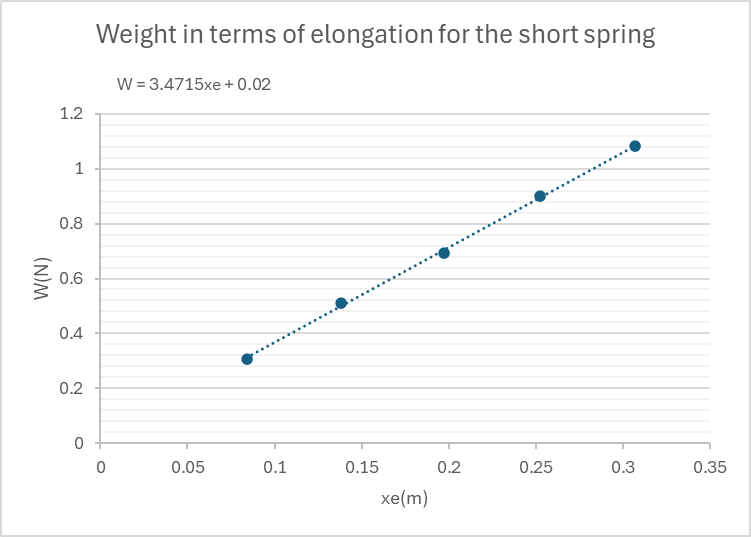
\includegraphics[width = 0.7\linewidth]{constant_short_spring.png}
    \caption{Weight as a function of elongation for the short spring}
\end{figure}
\begin{figure}[!h]
    \centering
    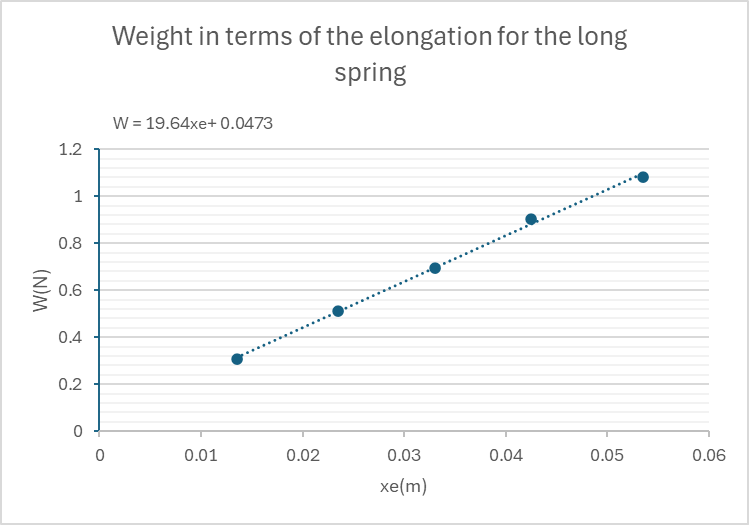
\includegraphics[width = 0.7\linewidth]{constant_long_spring.png}
    \caption{Weight as a function of elongation for the long spring}
\end{figure}
\subsection{Calculations}
Using the measured values, the spring constants can be determined. To determine
$x_e$ the following equation is used:
\begin{equation}
    x_e = l_1 - l_0
\end{equation}
To calculate the force that is applied to the spring, the weight equation is
used:
\begin{equation}
    W = mg
\end{equation}
By using equation \ref{eq:2} the spring constant can be therefore calculated.
\subsubsection{Example calucaltion}
By using the first data point of table \ref{tab:1}, the following calculations
are made to determine the spring constant.
\begin{gather*}
\intertext{Firstly, the weight of the discs and hook are calculated:} \\
 W = m \cdot g = 31.1~\mathrm{g} \cdot 0.001~\mathrm{\frac{g}{kg}} \cdot 9.81~\mathrm{\frac{kg}{N}} = 0.305091~\mathrm{N} \approx 0.31~\mathrm{N}\\
\intertext{Afterwards, the elongation is calculated:} \\
 x_e = l_1 - l_0 = 13.1~\mathrm{cm} - 4.7~\mathrm{cm} = 8.4~\mathrm{cm} \approx 0.08~\mathrm{m}\\
\intertext{Finally, the spring constant can be calculated using equation \ref{eq:2}:} \\
k x_e = W \Rightarrow k = \frac{W}{x_e} = \frac{0.305 ~\mathrm{N}}{0.084~\mathrm{m}} = 3.6309~\mathrm{Nm\inv} \approx 3.63~\mathrm{Nm\inv} 
\end{gather*}
\subsubsection{Error calculations}
As the mass was calculated using a digital scale, the uncertainty is the sum of
the smallest division(unc).
\[ \Delta m = 0.01~\mathrm{g} = 0.01~\mathrm{g} \cdot 10^{-3}~\mathrm{kg}\]
Since both $l_0$ and $l_1$ were measured using two markers on a ruler, the
uncertainty in the measurement is equal to half of the smallest division(unc).
\[ \Delta l_0 = \Delta l_1 = \frac{0.05~\mathrm{cm}}{2} = 0.025~\mathrm{cm} =
0.025 \cdot 10^{-2}~\mathrm{m} \]
\end{flushleft}
\end{document}